\documentclass{sig-alternate}
%[preprint]
% The following \documentclass options may be useful:
%
% 10pt          To set in 10-point type instead of 9-point.
% 11pt          To set in 11-point type instead of 9-point.
% authoryear    To obtain author/year citation style instead of numeric.

\makeatletter
%\def\@copyrightspace{\relax}
\makeatother


\usepackage{graphicx}
\usepackage{tikz}
%\usepackage{gnuplot-lua-tikz}
\usepackage{color}
\usepackage{tabularx}
\usepackage{fixltx2e}
%% \usepackage{dblfloatfix}
\usepackage{varwidth} % http://ctan.org/pkg/varwidth
\usepackage{listings}
\usepackage{url}
\usepackage{balance}
\usepackage{amsmath}
\usepackage{enumitem}
\usepackage{caption}

\lstset{
%  backgroundcolor=\color{yellow!20},%
  basicstyle=\small\ttfamily,%
  numbers=left, numberstyle=\tiny%
}

\newtheorem{thm}{Problem}
\newdef{definition}{Definition}
\DeclareMathAlphabet{\mathpzc}{OT1}{pzc}{m}{it}
\newtheorem{theorem}{Theorem}[section]
\newtheorem{lemma}[theorem]{Lemma}

\usepackage{xcolor}
\usepackage{framed}
\usepackage{amssymb,amsmath}
\usepackage{ifxetex,ifluatex}
\usepackage{fancyvrb}
\usepackage{comment}

\begin{document}

\title{\Large\bf Design Space Exploration for mriq accelerator}
\subtitle{\normalsize COMS E6901 2020 Summer Research}

\numberofauthors{1}
\author{
\alignauthor
Pei Liu\\
\vspace{0.2cm}
       \email{pl2748@columbia.edu}
}

\vspace{-2cm}

\maketitle

\vspace{-2cm}

\begin{abstract}
{\small\em
  This report focuses on design space exploration result over the previously designed accelerator for computing MRI-Q matrix.
}
\end{abstract}

%%%%%%%%%%%%%%%%%%%%%%%% Introduction %%%%%%%%%%%%%%%%%%%%%%%%%%%%%%%%%%%%%
\section{Introduction}
\label{sec:intro}
To prepare the mriq accelerator to go public release, we need to do some further work. For example, increase the configuration ability of this accelerator. The initially designed accelerator only works for the ``small" and ``medium" datasets from the Parboil benchmark, but not for the ``large" dataset in Table.~\ref{tab-1}. We also want this accelerator to work for any input image sizes.
\begin{table}[h!]
    \centering
    \begin{tabular}{c|c|c|c}
    \hline
       name  & image size & \# of pixels & K-space dimension  \\
    \hline
        small  & 32*32*32 & 32768 & 3072 \\
        medium & 64*64*64 & 262144 & 2048\\
        large & 128*128*128 & 2097152 & 2097152\\
        \hline
    \end{tabular}
    \caption{Datasets of MRIQ from Parboil Benchmark}
    \label{tab-1}
\end{table}

%%%%%%%%%%%%%%%%%%%%%%%% Specification %%%%%%%%%%%%%%%%%%%%%%%%%%%%%%%%%%%%%

\section{Specification}
\subsection{DSE plan to do}
\begin{enumerate}
\setlength\itemsep{-0.15em}
\item Try more extensive WL and IL range. Find the optimal WL and IL setting, which works for any random inputs.
\item Modifying compute kernel code to exploit loop unrolling.
\item Optimize the algorithm of sine function which is used in the compute kernel.
\item Use ``ping-pong" buffer to make the value of numX and numK both configurable.
\item Optimizing and defining PLM blocks to be configurable for any dataset sizes.
\item Split the input image among several accelerator instances on ESP for some enormous datasets.
\end{enumerate}

\subsection{Critical points}

\begin{enumerate}
\setlength\itemsep{-0.15em}
\item Organize various designs by editing the project.tcl, mriq\_directives.hpp, and memlist.txt files.

\end{enumerate}

%%%%%%%%%%%%%%%%%%%%%%%% Results %%%%%%%%%%%%%%%%%%%%%%%%%%%%%%%%%%%%%
\section{Results}
I have designed 12 different versions of accelerators. Two different architectures are exploited, which are A0 and A1. A0 represents that all the k-space data, which contains 5 variables, are stored in the PLM. A1 only loads a portion of k-space data into PLM at a time and uses a ping-pong buffer to make loading and computing, and storing processes in parallel. To accelerate the computation process, I have tried 3 different levels of parallelism on the computation kernel. Loop-unrolling and loop-pipelining are used at the same time, with loop unrolled for 4, 8, 16 times. Then this work has also exploited different DMA widths, 32 and 64. Each accelerator is represented as "P\#\_A\#\_dma\#". For example, P4\_A0\_dma64 represents this accelerator using architecture A0, loop unrolled 4 times and DMA width as 64. \\


\subsection{Datasets}

There are three datasets provided by the Parboil benchmark with different image resolutions, shown in Table.\ref{tab-1}. In addition to these three datasets, I have generated a test dataset out of ``small", which is used to do testing during the design phase. The configuration parameters for ``test" are much smaller than the above 3 datasets, with \# of pixels as 4 and k-space dimension as 16. The golden output for is provided by the Parboil benchmark. 

\subsection{Experiment setup}
 This designed accelerator is suitable to run any dataset. In project.tcl file, there are 4 testbenches, which are
 \begin{itemize}
 \setlength\itemsep{-0.15em}
     \item ``test" 
     \item ``32\_32\_32\_dataset"
     \item  ``64\_64\_64\_dataset"
     \item  ``128\_128\_128\_dataset"
 \end{itemize}
 As introduced above, ``test" is used for bare-metal simulation. We need to specify testbench in project.tcl file. To evaluate different designs by area and latency, I ran the different accelerators on ``32\_32\_32\_dataset" testbench. \\
 
 The parameters for two different architectural designs, A0 and A1, are shown in Table.\ref{tab-2}. Then I have generated and simulated RTL for different parallelism levels, different DMA widths, and different architectures. 
 \begin{table}[h!]
     \centering
     \begin{tabular}{c|c|c}
        \hline
          Configurable variables& A0 & A1  \\
         \hline
         numX & 256 & 256 \\
         \hline
         batch\_size\_x & 128 & 128 \\
         \hline
         num\_batch\_x & 2 & 2 \\
          \hline
         numK & 3072 & 3072 \\  
         \hline
         batch\_size\_k & 3072 & 1024 \\
         \hline
         num\_batch\_x & 1 & 3 \\
         \hline
     \end{tabular}
     \caption{Parameters of two different architectural designs}
     \label{tab-2}
 \end{table}
 

\subsection{Pareto Curve}
The area and latency data of each accelerator for architecture A0 and A1 drawn from HLS simulation and RTL simulation is shown in Fig.\ref{fig-1}. It has 12 dots, which are analyzed in the following sections. Each section shows how different design considerations affect their position in the Pareto curve. 
\begin{figure}[h!]
    \centering
    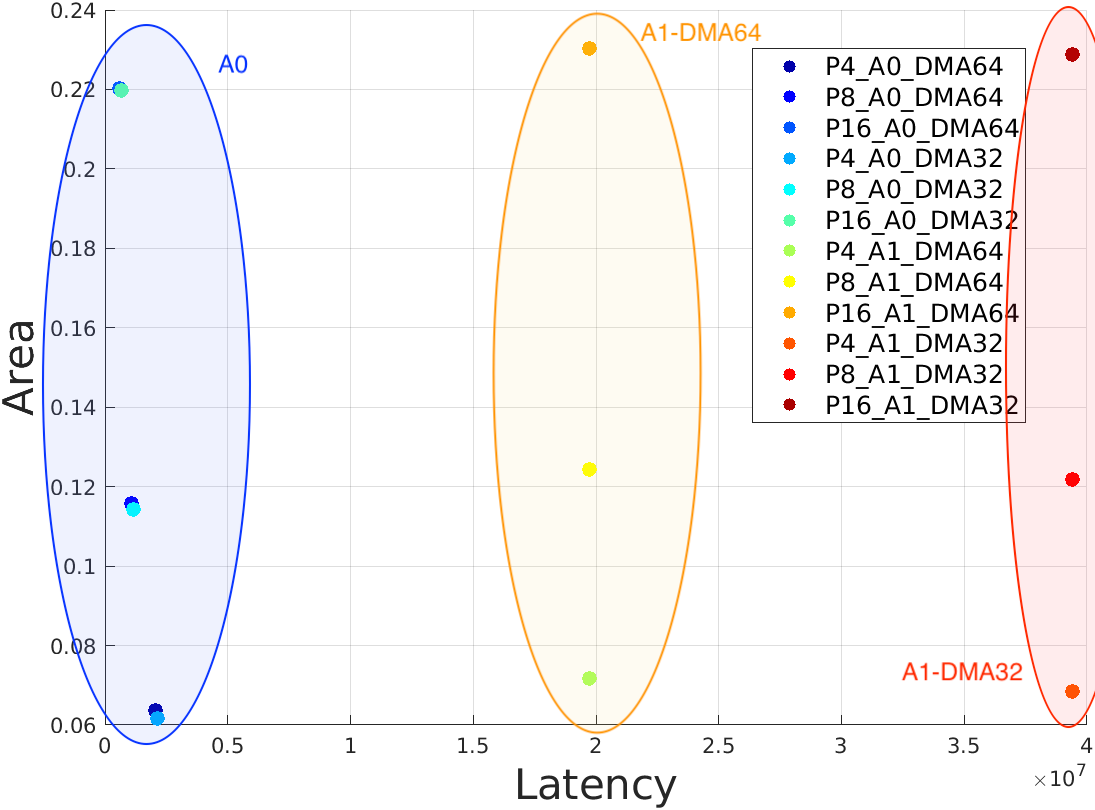
\includegraphics[width=0.85\columnwidth]{figure/result_all.png}
    \caption{Pareto curve of 12 designs}
    \label{fig-1}
\end{figure}


%%%%%%%%%%%%%Conclusions

\subsubsection{Architecture Type}
For the MRIQ application, the input data of one dataset can be divided into two groups. One group of data is coordinates information from frequency space, which is called k-space data. The other group is the sampling positions in three dimensional space, which is sometimes called sampling space data. There are 5 variables with size numK are from k-space, and 3 variables with size numX are from sampling space. To explain with dataset in Table.\ref{tab-1}, \# of pixels is numX and k-space dimension is numK. Each element of the Q matrix is a complex number, with imaginary and real part. One pair of output data is computed by using one point from sampling space and all the points in k-space. So the whole k-space data will be used for numX times while data from the sampling space is only used for once. For the three datasets introduced before, and any arbitrary dataset, we can store a part of data points from the sampling space, which will not damage latency. But as for the k-space data, it is highly reused. So it is desirable to store all the k-space data into PLM. \\

For the ``small" and ``medium" dataset, it has 15 K words at most for k-space data. If the data width is 32 bits, then the storage requirement is 60 K Bytes. We can store all the k-space data into PLM, For the ``large" dataset, it is 20 M words, which is 80 M Bytes. For some potential unknown applications with higher image resolution, the storage requirement for k-space data could be even larger. The storage cost may be so high that we want to sacrifice speed. For a specific application, the designer should balance the storage cost and speed requirements. For the MRI Q matrix application, the Q matrix computation is not in real-time, so we may want to save the cost of storage and compromise on speed.\\

For both A0 and A1, we only load a small part of sampling space data at a time. Because we notice that the computation of one output takes much longer time than loading one sampling space data. So we use ping-pong buffer to load sampling space data and do the computation and store output in a pipeline. When the accelerator can store all the k-space data, we load all k-space data first. But when k-space data size is too big for PLM size, we can only load portion of the k-space data into PLM and use ping pong buffer to parallelize loading process and computation process. In this design space exploration project, I have designed accelerators for both scenarios. A0 represents accelerator which stores all the k-space data into PLM, while A1 represents accelerators which only store a part of k-space data at a time. \\

Now we use the parameters shown in Table.\ref{tab-2}, and with parallelism level as 4. For A1, by looking at the RTL simulation waveform, we know that loading one k variable takes 5 $\mu$s and there are 5 k-space variables needs to be loading into PLM for every batch. So it takes 25 $\mu$s to load one batch of k-space data into PLM. Loading three batches takes 75 $\mu$s. By analyzing the waveform, we know that generating one pair of output data takes 77 $\mu$s. So the computation time is totally hidden in background. \\

A0 architecture loads all the k-space data into PLM. It uses ping pong buffer to load sampling space data. When batch\_size\_x is set to 128, the RTL simulation waveform shows that loading one batch of sampling space data takes 2 $\mu$s, generating one pair of output data takes 7 $\mu$s, and generating 128 pairs of output data takes 900 $\mu$s. So the computation time, including reading from PLM, is dominating, and the loading process of the sampling space data is hidden by computation process. \\

The comparison of latency performance of A0 and A1 is shown in Table.\ref{fig-3}. We can see that when loading the whole k-space data into PLM can reduce the latency by at least 90\% when compared with loading a portion of k-space data into PLM.

\begin{table}[ht!]
    \centering
    \begin{tabular}{c|c|c}
    \hline
    Accelerator & Latency & Improvement \\
    \hline
    P4\_A1\_DMA64  &  19754540 &      \\                                        
    P4\_A0\_DMA64  &  2077060 &       -89.49\% \\                               
    \hline
    P8\_A1\_DMA64  &  19753260 &      \\
    P8\_A0\_DMA64  &  1096580  &      -94.45\% \\
    \hline
    P16\_A1\_DMA64  & 19752640 &      \\
    P16\_A0\_DMA64  & 607620  &      -96.92\% \\
    \hline
    \end{tabular}
    \caption{Latency Data for A0 and A1}
    \label{tab-3}
\end{table}
%%%%%%%%%%%%%%%%%

\subsubsection{DMA width}
When the accelerator is more memory-bound, which is A1, DMA width has bigger influence on latency. In Fig.\ref{fig-1}, A1 architecture, latency values of accelerator with DMA width as 64 are highlighted with a yellow circle, while those with DMA width as 32 are in red circle. Increasing DMA width of A1 architecture from 32 to 64 can reduce latency by almost 50\% while keeping area almost the same. Since the memory time is dominating computation time for A1 architecture, the loading process is twice faster when DMA width changing from 32 to 64. The data for A1 architecture in Fig.\ref{fig-1} is also shown in Table.\ref{tab-4}. \\

\begin{table}[ht!]
    \centering
    \begin{tabular}{c|c|c}
    \hline
    Accelerator & Latency & Improvement \\
    \hline
    P4\_A1\_DMA32 &     39421740     & \\
    P4\_A1\_DMA64       &   19754540         & -49.89\% \\
    \hline
    P8\_A1\_DMA32       &   39420460         & \\
    P8\_A1\_DMA64       &   19753260         & -49.89\% \\
    \hline
    P16\_A1\_DMA32 &  39419840       & \\
    P16\_A1\_DMA64 &  19752640       & -49.89\% \\
    \hline
    \end{tabular}
    \caption{Latency Data for Different DMA widths of A1}
    \label{tab-4}
\end{table}
\\
So when a dataset is too big to fit into PLM, the optimization direction of performance is to accelerate data transportation process. Optimizing computation process would benefit very little to the whole performance. When all data can be stored in PLM, this accelerator is more computation bounded. The result of memory time improvement still can accelerate the application, but with less contribution. Table.\ref{tab-5} shows that the biggest improvement for A0 is 11.63\%. 

\begin{table}[ht!]
    \centering
    \begin{tabular}{c|c|c}
    \hline
    Accelerator & Latency & Improvement \\
    \hline
    P4\_A0\_DMA32 & 2157060      & \\
    P4\_A0\_DMA64 &  2077060 &       -3.71\%   \\                                    \hline
    P8\_A0\_DMA32 &  1176580 &       \\                         
    P8\_A0\_DMA64 &  1096580 &       -6.80\%   \\                             
    \hline
    P16\_A0\_DMA32 &  687620 &       \\                                 
    P16\_A0\_DMA64 &  607620 &       -11.63\%   \\ 
    \hline
    \end{tabular}
    \caption{Latency Data for Different DMA widths of A0}
    \label{tab-5}
\end{table}




\subsubsection{Parallelism}

We have discussed in ``PLM size" section that A1 architecture is more memory bound while A0 is more computation bound. The latency for A0 is shown in Table.\ref{tab-6} and Fig.\ref{fig-2}, while latency for A1 is shown in Table.\ref{tab-7} and Fig.\ref{fig-3}


\begin{figure}[h!]
    \centering
    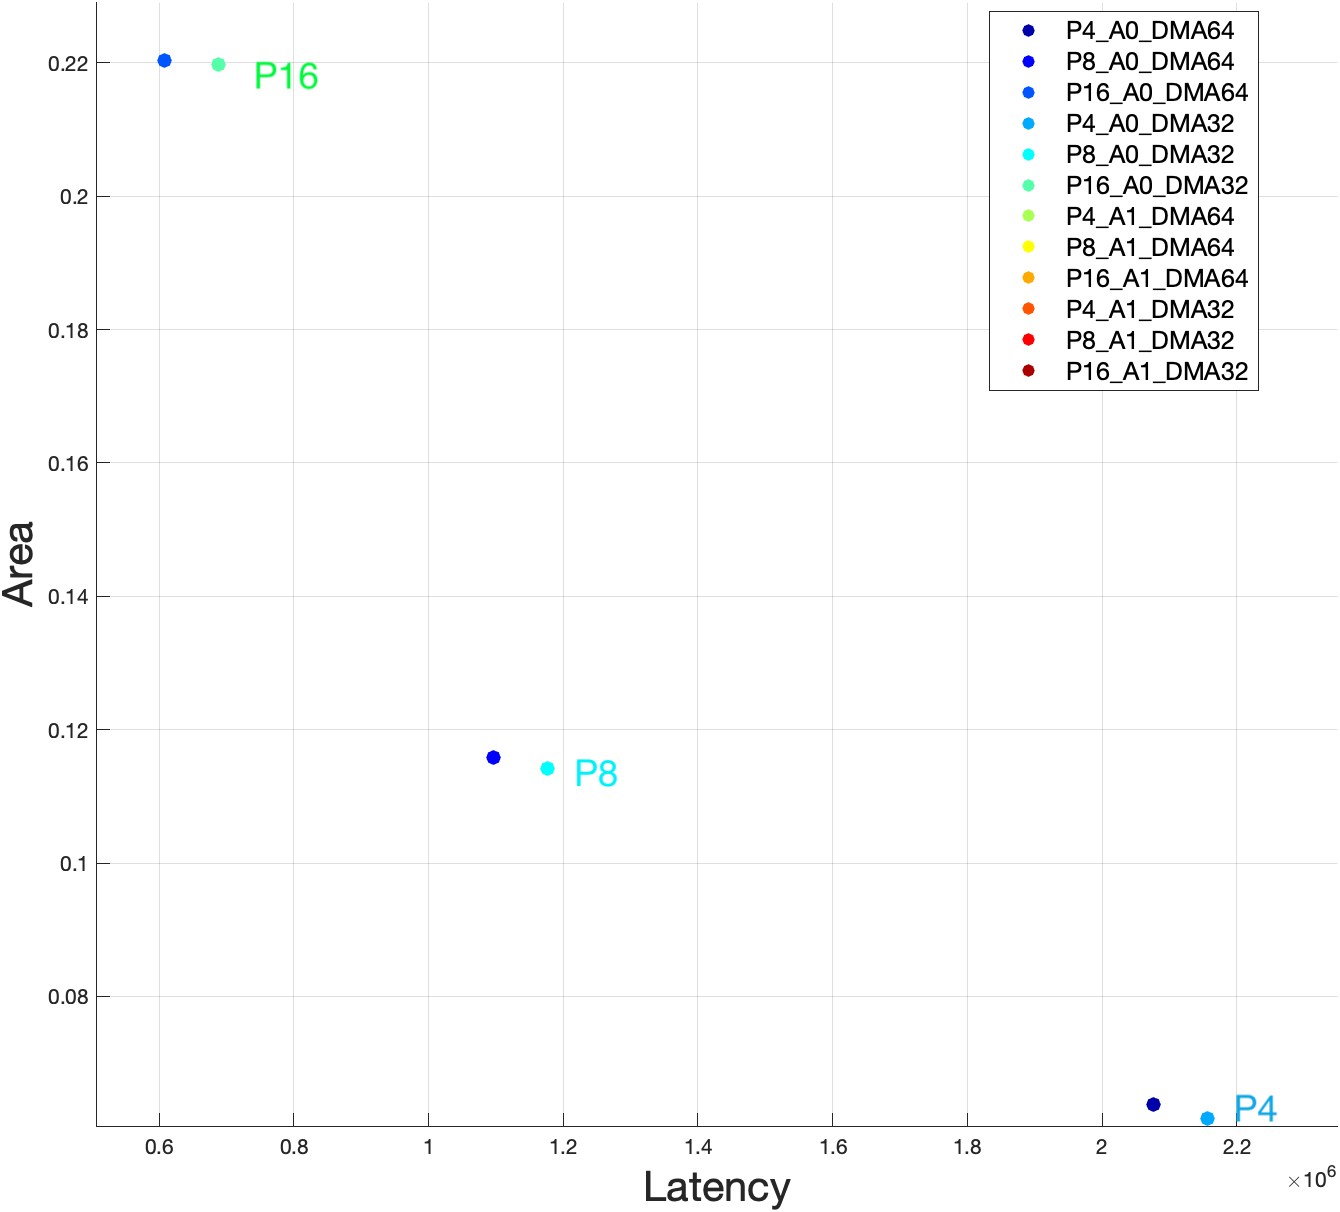
\includegraphics[width=0.85\columnwidth]{figure/result_A0.png}
    \caption{Pareto curve of 6 designs of A0}
    \label{fig-2}
\end{figure}

\begin{figure}[h!]
    \centering
    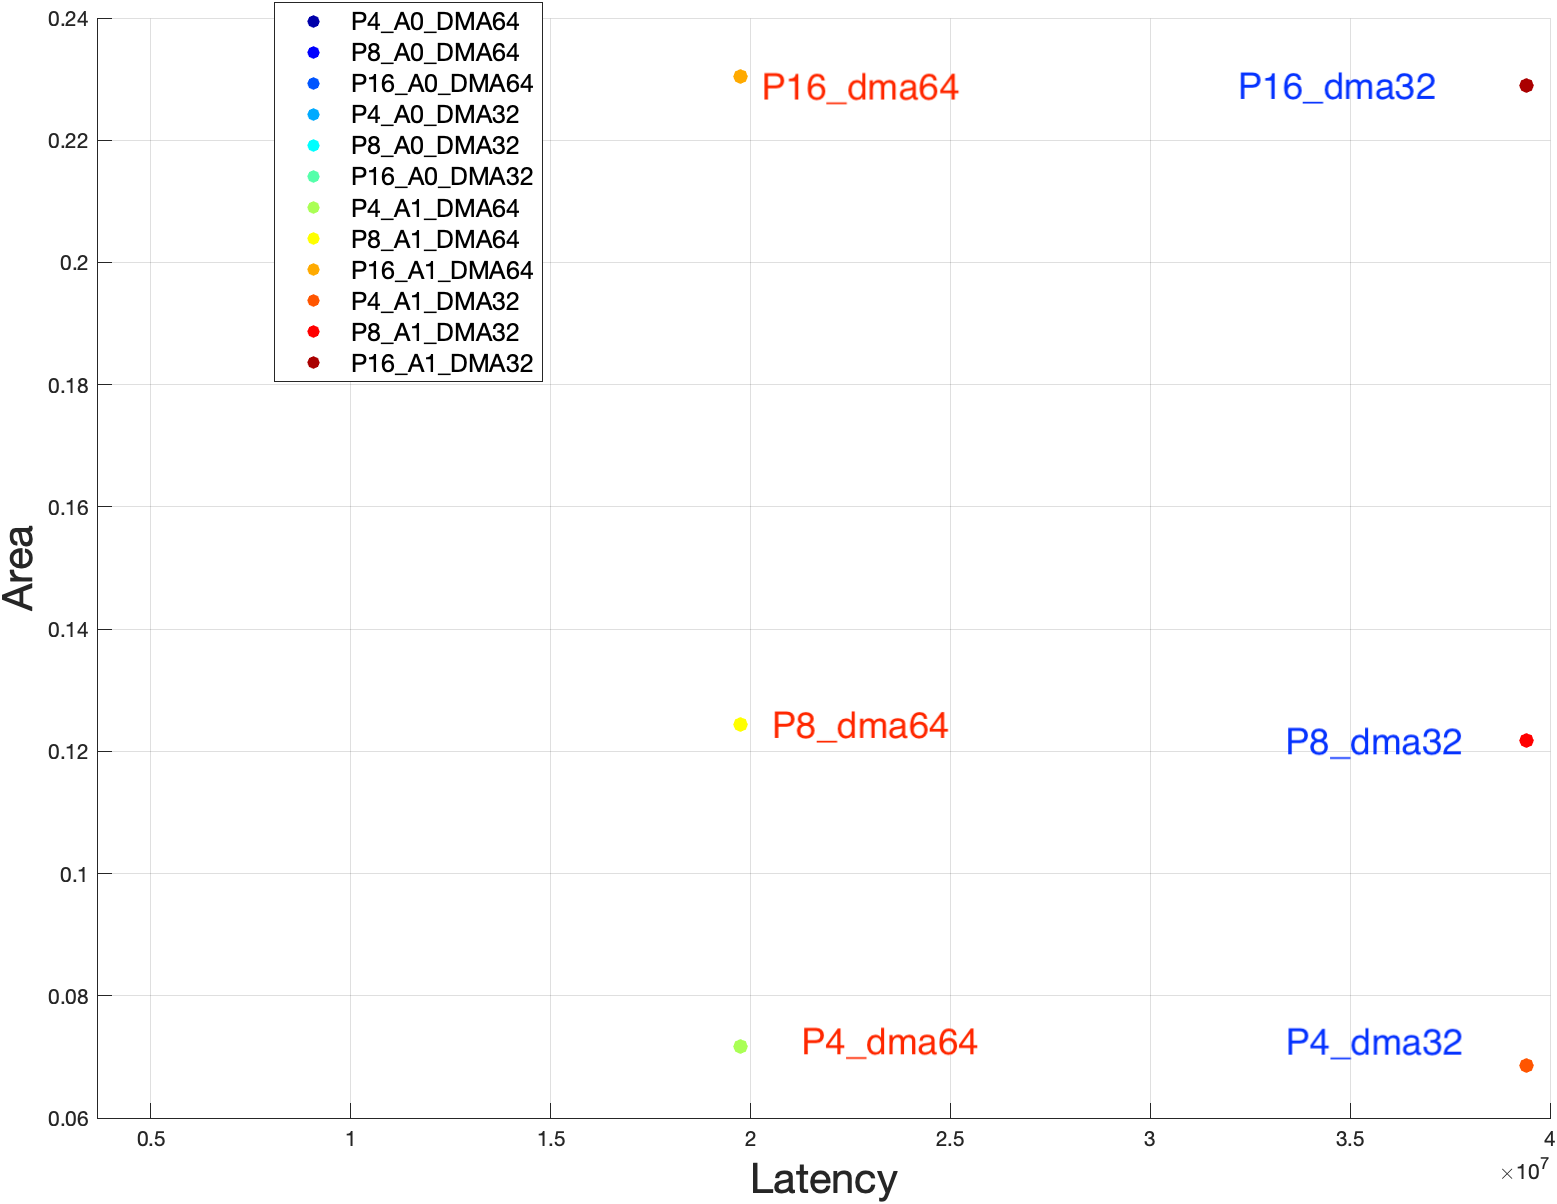
\includegraphics[width=0.85\columnwidth]{figure/result_A1.png}
    \caption{Pareto curve of 6 designs of A1}
    \label{fig-3}
\end{figure}

\begin{table}[ht!]
    \centering
    \begin{tabular}{c|c|c}
    \hline
    Accelerator & latency & Improvement \\
    \hline
    P4\_A0\_DMA64  &    2077060   & - \\
    P8\_A0\_DMA64  &    1096580	  &  -47.2\% \\
    P16\_A0\_DMA64  &   607620    &  -44.6\% \\
    \hline
    \end{tabular}
    \caption{Latency Data for Different Parallelism Level of A0}
    \label{tab-6}
\end{table}

\begin{table}[ht!]
    \centering
    \begin{tabular}{c|c|c}
    \hline
    Accelerator & latency & Improvement \\
    \hline
    P4\_A1\_DMA64  &    19754540    & - \\
    P8\_A1\_DMA64  &    19753260	  &  -0.006\% \\
    P16\_A1\_DMA64  &   19752640    &  -0.003\% \\
    \hline
    \end{tabular}
    \caption{Latency Data for Different Parallelism Level of A1}
    \label{tab-7}
\end{table}

In order to improve latency, I used loop-unroll and loop-pipeline in computation process. For architecture A0, computation pseudo code is shown in Fig.\ref{fig-4}. The inner for loop is unrolled for a certain number, where 4, 8, 16 are implemented. The reading from PLM procedure, computation, and accumulating can be pipelined. The same design logic is also used for architecture A1, but the max iteration of the outer for loop is batch\_size\_k instead of numK.

\begin{figure}[h!]
    \centering
    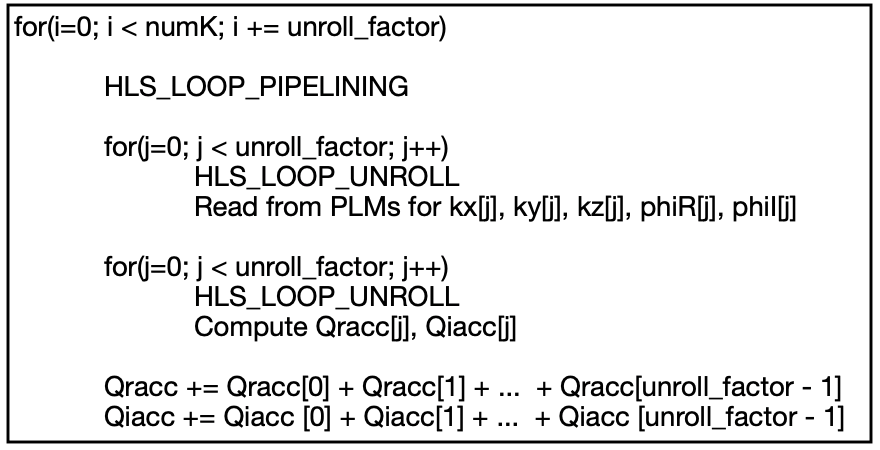
\includegraphics[width=0.85\columnwidth]{figure/pseudo code.png}
    \caption{Pseudo code of for loop unrolling and pipelining}
    \label{fig-4}
\end{figure}


\subsubsection{Fixed point datatype optimization}

I use two kinds of datatype for this accelerator: FPDATA\_S and FPDATA\_L. FPDATA\_S represents small data and FPDATA\_L represents large data. By looking at the input data, output data and intermediate results, I noticed that some data are bound to be very small value, for example, the output of trigonometric functions is always less than 1, and some are large values. The range of data are shown in Table.\ref{tab-8}. Then, for small values, such as (kx, ky, kz, phiR, phiI, x, y, z, and phiMag, sinArg, cosArg), setting Integer\_Length (IL) as 6, and Word Length (WL) as 24, for large values setting IL as 11 and WL as 24 can satisfy representation of all data without error. on both "small" and "middle" dataset.\\
The definition of these two fixed-point are as follows:\\
\\
\\
const unsigned int FPDATA\_S\_WL = 24;\\
const unsigned int FPDATA\_S\_IL = 6;\\
typedef cynw\_fixed<FPDATA\_S\_WL, FPDATA\_S\_IL, SC\_RND> FPDATA\_S;\\
\\
const unsigned int FPDATA\_L\_WL = 24;\\
const unsigned int FPDATA\_L\_IL = 11;\\
typedef cynw\_fixed<FPDATA\_L\_WL, FPDATA\_L\_IL, SC\_RND> FPDATA\_L;\\
\\

\begin{table}[ht!]
    \centering
    \begin{tabular}{c|c|c|c}
    \hline \hline
   Variables &       Max&    Min& Integer bits\\
   \hline \hline
 x&     3.083235        &-0.500000& 3 \\
 y&     0.484375        &-0.500000& 1 \\
 z&     0.484375        &-0.500000& 1 \\
 kx&    10.889303       &-10.889303& 5 \\
 ky&    16.019472       &-16.019472& 5 \\
 kz&    0.585179        &-0.585179& 1\\
 phiI   &0.484375       &0.312500& 0 \\
 phiR   &0.484375       &0.406250& 0 \\
 phiMag &0.469238       &0.262695& 0 \\
 cosArg&        1.000000        &-1.000000& 2\\
 sinArg &1.000000       &-1.000000& 2 \\
 \hline
 expArg &226.168869     &-226.168869& 9 \\
 Qracc  &961.000000     &-472.693146& 11 \\
 Qiacc  &97.710320      &-97.710320& 8 \\
\hline \hline
    \end{tabular}
    \caption{Value range for all variables}
    \label{tab-8}
\end{table}

The result shows that the error rate is 0.17\% when error threshold (percentage difference between computed output and golden output), is set as 5\%. For those percentage difference larger than 5\%, the output data, golden output, and percentage difference are shown in Table.\ref{tab-9}. We can see that the percentage differences between each pair are less than 100\%. This MRI-Q accelerator is comparing the exact values. Since Q matrix computation is only one phase of image reconstruction, so it might tolerate a certain level of errors for Q matrix values. So we the data width can be reduced to 24 compared to 32 to improve latency and area at the same time.

\begin{table}[ht!]
    \centering
    \begin{tabular}{c|c|c}
    \hline
Golden  & Out       &percentage\_difference \\
\hline
-0.014945& -0.013428&  10.15\% \\                                                                            
0.010379 & 0.014160  & 36.43\% \\                                                                           
0.071230 & 0.078247  & 9.85\% \\                                                                            
0.051077 & 0.057251  & 12.09\% \\                                                                           
-0.011609& -0.009644 & 16.93\% \\                                                                          
0.003671 & 0.005737  & 56.28\% \\                                                                           
-0.013043 &-0.006470 &  50.39\% \\    
\hline
    \end{tabular}
    \caption{Errors for 4096 outputs}
    \label{tab-9}
\end{table}











\subsection{FPGA Prototyping and Lantency Test}
I have tested latency of hardware execution, and the software running time for each dataset by invoking linux on FPGA, shown in Fig.\ref{fig-f}. We have discussed before that for "small" and "middle" dataset, the whole K-space data is loaded into PLM. So the testing for these two datasets is done only for A0 architecture. For the "large" dataset, loading dataset to FPGA is so slow that I generated different sizes of data from the "128x128x128" dataset and tested them to see the trend of latency.\\

\begin{figure}[h!]
    \centering
    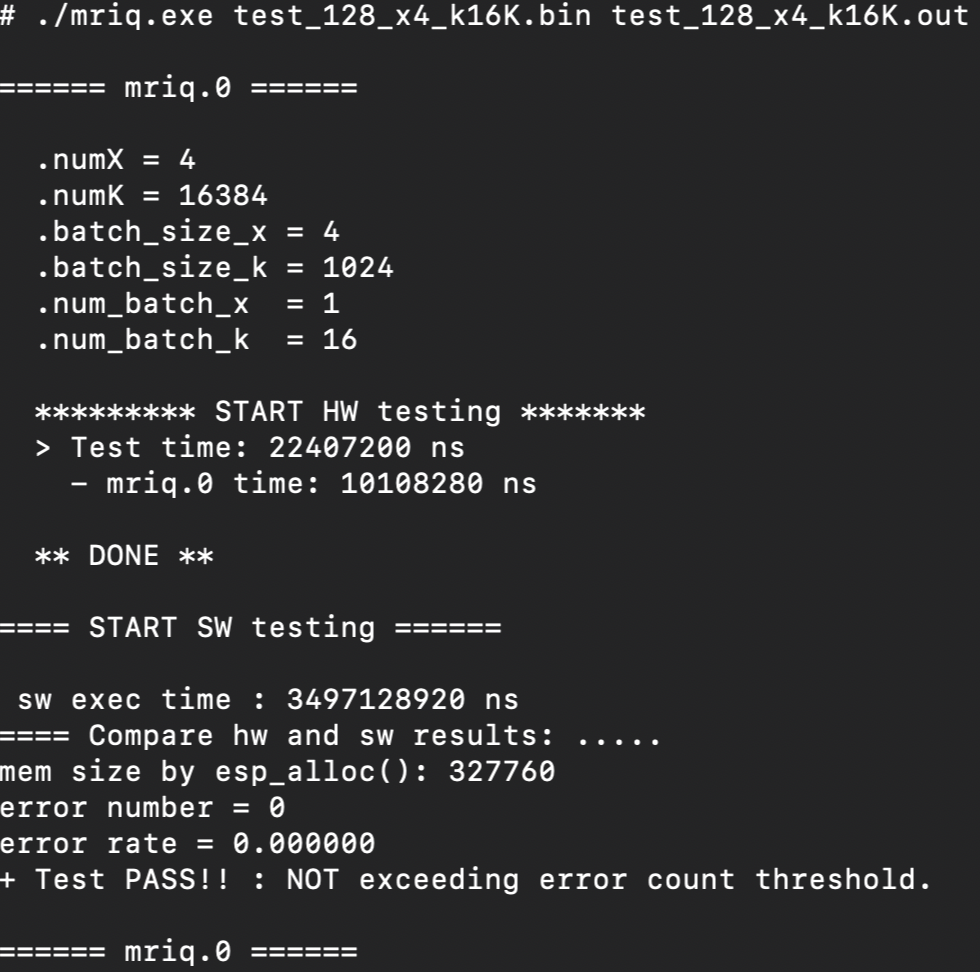
\includegraphics[width=0.85\columnwidth]{figure/fpga-proto.png}
    \caption{Running linux application on FPGA}
    \label{fig-f}
\end{figure}

For A0 architecture, data is shown in Fig.\ref{fig-d32} and Fig.\ref{fig-d64} for 32x32x32 and 64x64x64 dataset, respectively. The testing is running on Ariane core with DMA width as 64. Fig.\ref{fig-d32-64} shows that comparison. The x-axis shows three parallel level in compute process. For A0 architecture, increasing parallelism in compute can improve latency, as we discussed the synthesis result in section 3.3. 


\begin{figure}[h!]
    \centering
    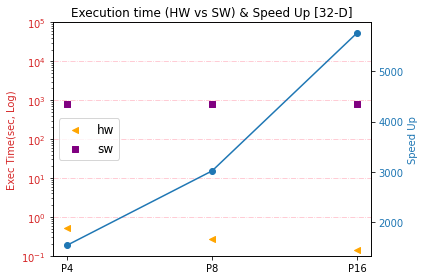
\includegraphics[width=0.85\columnwidth]{figure/D32-SW-HW.png}
    \caption{Latency of 32x32x32 Dataset}
    \label{fig-d32}
\end{figure}

\begin{figure}[h!]
    \centering
    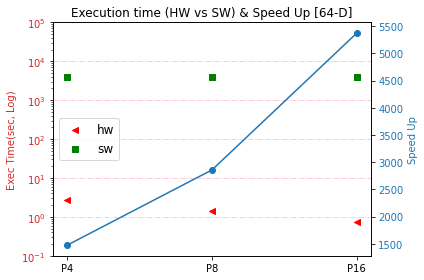
\includegraphics[width=0.85\columnwidth]{figure/D64-SW-HW.png}
    \caption{Latency of 64x64x64 Dataset}
    \label{fig-d64}
\end{figure}

\begin{figure}[h!]
    \centering
    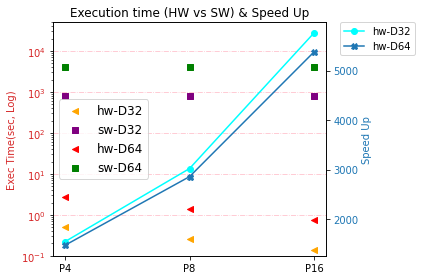
\includegraphics[width=0.85\columnwidth]{figure/D32-D64-HW-SW.png}
    \caption{Latency comparison of D32 and D64 Dataset}
    \label{fig-d32-64}
\end{figure}

For A1 architecture, latency results are shown in Fig.\ref{fig-a1-x} and Fig.\ref{fig-a1-k}. For 128x128x128 dataset, numX = numK = 2048K. To evaluation the speedup of accelerator with A1 architecture, I tested P4\_A1\_dma64. As we discussed in section 3.3, we know that parallel level in compute process won't affect latency performance, so it is good enough to choose the P4 accelerator (We should design an accelerator with parallelism level in computation process smaller than 4 which can also balance the loading and computing processes to further reduce area when with the same performance).

\begin{figure}[h!]
    \centering
    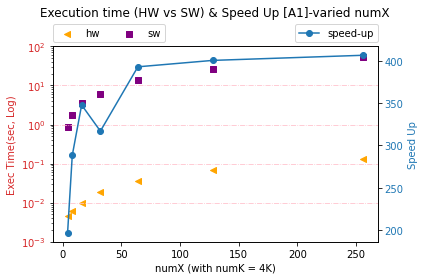
\includegraphics[width=0.85\columnwidth]{figure/K-4K-X-vary.png}
    \caption{Latency with varying numX (numK=4K)}
    \label{fig-a1-x}
\end{figure}

\begin{figure}[h!]
    \centering
    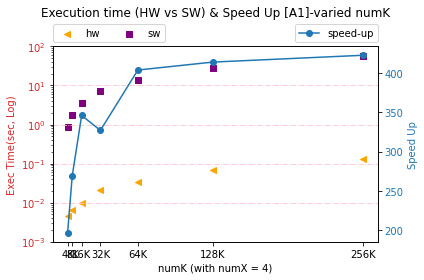
\includegraphics[width=0.85\columnwidth]{figure/X-4-K-vary.png}
    \caption{Latency with varying numK (numX=4)}
    \label{fig-a1-k}
\end{figure}

The speedup value is increasing when increasing the data size. At some point, speedup increasing is becoming smaller. Suppose it saturates. Then we get at least 400 times speed up compared with software execution.

\section{Conclusion}

\end{document}
